% begin module volumes-Cavelieri
\begin{frame}
\frametitle{Cavalieri's principle}
 {\it{Solids with equal cross-sectional areas have equal volume.}} \\
It is often illustrated convincingly with two stacks of coins. 

\begin{center}
{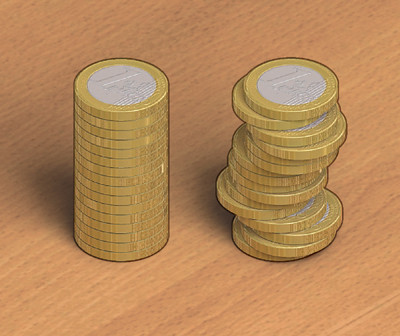
\includegraphics[width=.3\textheight]{volumes/pictures/v1}}
\end{center}

 Our formula 
\[
V=\int_a^bA(x)dx
\]
implies the truth of Cavalieri's principle, since the volumes $V$ are certainly 
equal if the cross-sectional areas $A(x)$ are equal.

\end{frame}


